\documentclass{article}
\usepackage{tikz}
\usepackage{amsmath}

\begin{document}

Un sistema lineare di due variabili $x$ e $y$ è un sistema di equazioni della seguente forma 
$$
\begin{cases}
    a\cdot x + b \cdot y = l\\
    c \cdot x + d \cdot y = m
\end{cases}
$$
dove $a,b,c,d, l,m$ sono numeri reali qualsiasi e $x$ e $y$ sono le incognite. 

Esempio

$$
\begin{cases}
     x + 2 \cdot y = 1\\
    3 \cdot x + 5 \cdot y = 4
\end{cases}.
$$
I sistemi di due variabili hanno una interessante interpretazione geometrica. Infatti, è noto che $ax + by = l$ è l'equazione di una retta nel piano, mettendo due equazioni a sistema si sta cercando l'eventuale intersezione di queste due rette del piano.  

\begin{center}
    \begin{tikzpicture}
        \draw[->] (-2,0) -- (4,0) node[right] {$x$};
        \draw[->] (0,-2) -- (0,4) node[above] {$y$};
        \draw[domain=-2:3, smooth, variable=\x, red] plot ({\x},{(1-\x)/2}) node[right] {$x + 2y = 1$};
        \draw[domain=-1:2, smooth, variable=\x, blue] plot ({\x},{(4-3*\x)/5}) node[right] {$3x + 5y = 4$};
    \end{tikzpicture}
\end{center}

Immaginare geometricamente il sistema può aiutare a ricordare meglio i tre casi a cui ci si trova di fronte risolvendo un sistema:
- impossibile 
- unica soluzione
- infinite soluzioni o indeterminato.

Infatti, il sistema è impossibile quando le rette corrispondenti sono parallele; è indeterminato quando le rette sono coincidenti.

\begin{center}
    \begin{tikzpicture}
        \draw[->] (-2,0) -- (4,0) node[right] {$x$};
        \draw[->] (0,-2) -- (0,4) node[above] {$y$};
        \draw[domain=-2:3, smooth, variable=\x, red] plot ({\x},{(1-\x)/2}) node[right] {Retta 1};
        \draw[domain=-2:3, smooth, variable=\x, red, dashed] plot ({\x},{(3-\x)/2}) node[right] {Retta 2 (parallela)};
    \end{tikzpicture}
    
    \begin{tikzpicture}
        \draw[->] (-2,0) -- (4,0) node[right] {$x$};
        \draw[->] (0,-2) -- (0,4) node[above] {$y$};
        \draw[domain=-2:3, smooth, variable=\x, red] plot ({\x},{(1-\x)/2}) node[right] {Retta 1};
        \draw[domain=-2:3, smooth, variable=\x, red] plot ({\x},{(1-\x)/2}) node[right] {Retta 2 (coincidente)};
    \end{tikzpicture}
\end{center}

Gli strumenti principali per capire in quali dei tre casi ci si trova in due variabili sono tre:

\begin{enumerate}
    \item  Verificare se le rette corrispondenti alle equazioni sono parallele.
    \item Il criterio del determinante per essere in grado di usare Rouche-Capelli.

    \item Applicare correttamente il metodo di sostituzione, del confronto o di Gauss. Se durante il procedimento hai ottenuto una uguaglianza non vera come $- 1 = 0$ allora il sistema è impossibile. Se hai trovato un'equazione $0 = 0$, allora il sistema è indeterminato. Se invece hai trovato un'unica soluzione, il sistema è risolvibile. 
\end{enumerate}

\textbf{Osservazione 1:}
Per controllare se due rette sono parallele o coincidenti è di aiuto questo trucco provare a ricondursi alla stessa equazione. Penso che risulteranno più chiari due esempi anziché usare lettere e distinguere in casi.
Esempio rette coincincidenti, sistema indeterminato: 
$$
\begin{cases}
2x + 6y = 2
x + 3y = 1
\end{cases}
$$
Raccogliendo $2$ nella prima equazione si ottiene
$$
\begin{cases}
    2 \cdot ( x + 3 y ) = 2\cdot 1 \\
    x + 3 y = 1
\end{cases}
$$
Ci siamo accorti che la prima equazione è equivalente alla seconda! Detto altrimenti, la prima e la seconda equazione rappresentano la stessa retta, di conseguenza siamo nel caso di due rette coincidenti, ossia sistema indeterminato

\paragraph{}
Esempio rette parallele, sistema impossibile:

Raccogliendo $3$ nella prima equazione si ottiene
\begin{cases}
    3x + 9 y = 1 \\
    x + 3 y = 1
\end{cases}
dividendo per $3$ la prima equazione si ottiene

\begin{cases}
    x + 3 y = \dfrac{1}{3} \\
    x + 3 y = 1
\end{cases}
abbiamo ottenuto le equazioni di due rette parallele. Infatti, dall'ultimo sistema è facile verificare che le due rette hanno lo stesso coefficiente angolare ma intercette diverse.

\paragraph{}
\textbf{NB:}
Potreste avere noto che i passaggi nell'osservazione sopra sono passaggi che possono essere inclusi nel metodo di Gauss. Questo è un piccolo spoiler su quello che viene dopo: si potrebbe dire, esagerando un pochino, che tutti i moderni i metodi diretti per la determinazione dei sistemi lineari sono una variante migliorata del metodo di Gauss.


\textbf{Osservazione 2:}
Per i casi con più variabili in genere si utilizza il criterio del determinante per applicare il teorema Rouché-Capelli.

\textbf{Curiosità:}
Tutte le tecniche più avanzate nate per la risoluzione dei sistemi lineari sono raccolte sotto il nome di Algebra Lineare, una delle teorie matematiche più di successo di sempre. Applicata dalla fisica all'informatica e al centro della moderna rivoluzione delle reti neurali!

\paragraph{}
Di seguito ho spiegato i metodi di risoluzione dei sistemi lineari dando per scontato che il sistema fosse risolubile. Per adattare i metodi di sostituzione, del confronto e di Gauss agli altri casi, seguire le indicazioni sopra.

\section*{Risoluzione di un sistema lineare con il metodo di sostituzione}

Consideriamo il sistema:
\begin{equation*}
\begin{cases}
2x + 2y = 5 \\
3x - 4y = 1
\end{cases}
\end{equation*}

\subsection*{Passaggi}

\begin{enumerate}
    \item Isoliamo una variabile in un'equazione (scegliamo la prima):
    \begin{equation*}
        2y = 5 - 2x \quad \Rightarrow \quad y = \frac{5 - 2x}{2}
    \end{equation*}
    
    \item Sostituiamo nella seconda equazione:
    \begin{equation*}
        3x - 4\left(\frac{5 - 2x}{2}\right) = 1
    \end{equation*}
    
    \item Moltiplichiamo per semplificare:
    \begin{equation*}
        3x - \frac{20 - 8x}{2} = 1
    \end{equation*}
    
    \item Moltiplichiamo tutto per 2 per eliminare i denominatori:
    \begin{equation*}
        6x - (20 - 8x) = 2
    \end{equation*}
    
    \item Semplifichiamo:
    \begin{equation*}
        6x - 20 + 8x = 2 \quad \Rightarrow \quad 14x = 22 \quad \Rightarrow \quad x = \frac{11}{7}
    \end{equation*}
    
    \item Sostituiamo $x$ nella prima equazione per trovare $y$:
    \begin{equation*}
        y = \frac{5 - 2(\frac{11}{7})}{2} = \frac{35 - 22}{14} = \frac{13}{14}
    \end{equation*}


\end{enumerate}

\textbf{Risultato:} $x = \frac{11}{7}$, $y = \frac{13}{14}$
    

\begin{center}
    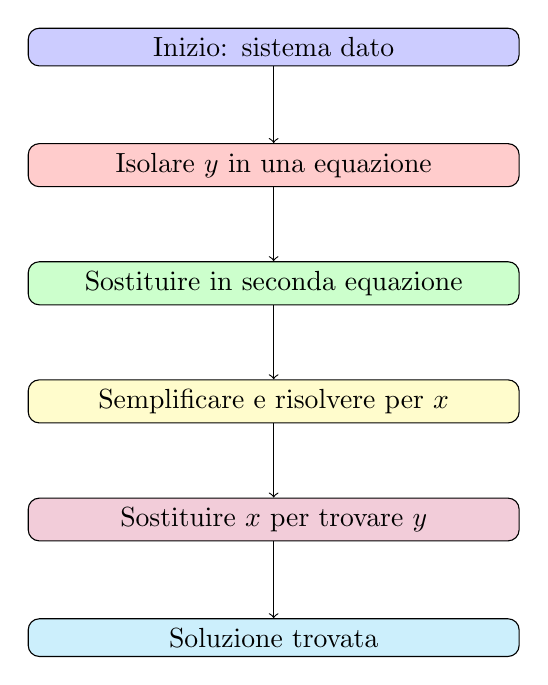
\begin{tikzpicture}[node distance=1.5cm, every node/.style={draw, rectangle, rounded corners, align=center, fill=blue!20, text width=6cm}]
        \node (start) {Inizio: sistema dato};
        \node (isola) [below of=start, fill=red!20] {Isolare $y$ in una equazione};
        \node (sostituisci) [below of=isola, fill=green!20] {Sostituire in seconda equazione};
        \node (semplifica) [below of=sostituisci, fill=yellow!20] {Semplificare e risolvere per $x$};
        \node (trovaY) [below of=semplifica, fill=purple!20] {Sostituire $x$ per trovare $y$};
        \node (fine) [below of=trovaY, fill=cyan!20] {Soluzione trovata};
        
        \draw[->] (start) -- (isola);
        \draw[->] (isola) -- (sostituisci);
        \draw[->] (sostituisci) -- (semplifica);
        \draw[->] (semplifica) -- (trovaY);
        \draw[->] (trovaY) -- (fine);
    \end{tikzpicture}
\end{center}


\subsection*{Metodo del Confronto}

\begin{enumerate}
    \item Esplicitiamo $y$ in entrambe le equazioni:
    \begin{equation*}
        y = \frac{5 - 2x}{2}, \quad y = \frac{3x - 1}{4}
    \end{equation*}
    \item Confrontiamo le due espressioni:
    \begin{equation*}
        \frac{5 - 2x}{2} = \frac{3x - 1}{4}
    \end{equation*}
    \item Risolviamo per $x$:
    \begin{equation*}
        4(5 - 2x) = 2(3x - 1)
    \end{equation*}
    \begin{equation*}
        20 - 8x = 6x - 2
    \end{equation*}
    \begin{equation*}
        20 + 2 = 6x + 8x \Rightarrow 22 = 14x \Rightarrow x = \frac{11}{7}
    \end{equation*}
    \item Sostituiamo in una delle equazioni:
    \begin{equation*}
        y = \frac{5 - 2(\frac{11}{7})}{2} = \frac{13}{14}
    \end{equation*}
\end{enumerate}

\begin{center}
    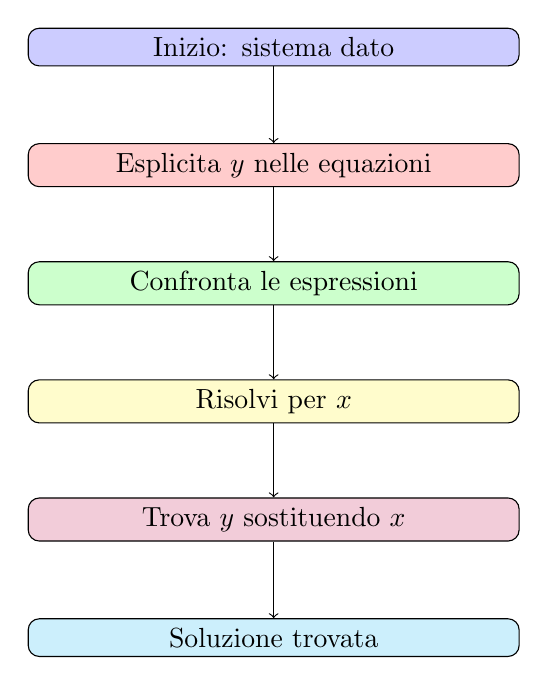
\begin{tikzpicture}[node distance=1.5cm, every node/.style={draw, rectangle, rounded corners, align=center, fill=blue!20, text width=6cm}]
        \node (start) {Inizio: sistema dato};
        \node (esplicita) [below of=start, fill=red!20] {Esplicita $y$ nelle equazioni};
        \node (confronta) [below of=esplicita, fill=green!20] {Confronta le espressioni};
        \node (risolvi) [below of=confronta, fill=yellow!20] {Risolvi per $x$};
        \node (trovaY) [below of=risolvi, fill=purple!20] {Trova $y$ sostituendo $x$};
        \node (fine) [below of=trovaY, fill=cyan!20] {Soluzione trovata};
        
        \draw[->] (start) -- (esplicita);
        \draw[->] (esplicita) -- (confronta);
        \draw[->] (confronta) -- (risolvi);
        \draw[->] (risolvi) -- (trovaY);
        \draw[->] (trovaY) -- (fine);
    \end{tikzpicture}
\end{center}


\subsection*{Metodo di Gauss}

\begin{enumerate}
    \item Scriviamo il sistema in forma matriciale:
    \begin{equation*}
        \left[\begin{array}{cc|c} 2 & 2 & 5 \\ 3 & -4 & 1 \end{array}\right]
    \end{equation*}
    \item Effettuiamo il pivoting sulla prima colonna dividendo la prima riga per 2:
    \begin{equation*}
        \left[\begin{array}{cc|c} 1 & 1 & 2.5 \\ 3 & -4 & 1 \end{array}\right]
    \end{equation*}
    \item Eliminazione: sottraiamo 3 volte la prima riga alla seconda:
    \begin{equation*}
        \left[\begin{array}{cc|c} 1 & 1 & 2.5 \\ 0 & -7 & -6.5 \end{array}\right]
    \end{equation*}
    \item Risolviamo per $y$ dalla seconda equazione:
    \begin{equation*}
        y = \frac{-6.5}{-7} = \frac{13}{14}
    \end{equation*}
    \item Sostituiamo il valore di $y$ nella prima equazione:
    \begin{equation*}
        x + \frac{13}{14} = 2.5
    \end{equation*}
    \begin{equation*}
        x = 2.5 - \frac{13}{14} = \frac{11}{7}
    \end{equation*}
\end{enumerate}

\begin{center}
    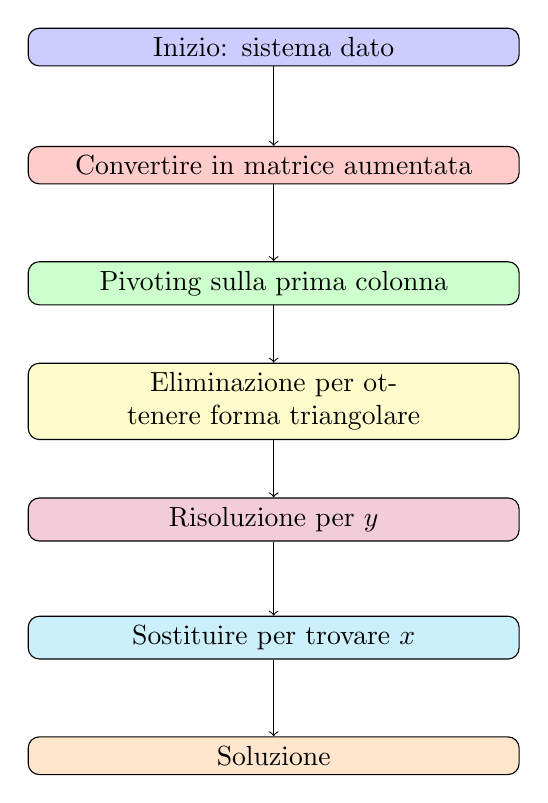
\begin{tikzpicture}[node distance=1.5cm, every node/.style={draw, rectangle, rounded corners, align=center, fill=blue!20, text width=6cm}]
        \node (start) {Inizio: sistema dato};
        \node (matrice) [below of=start, fill=red!20] {Convertire in matrice aumentata};
        \node (pivot) [below of=matrice, fill=green!20] {Pivoting sulla prima colonna};
        \node (eliminazione) [below of=pivot, fill=yellow!20] {Eliminazione per ottenere forma triangolare};
        \node (trovaY) [below of=eliminazione, fill=purple!20] {Risoluzione per $y$};
        \node (trovaX) [below of=trovaY, fill=cyan!20] {Sostituire per trovare $x$};
        \node (fine) [below of=trovaX, fill=orange!20] {Soluzione};
        
        \draw[->] (start) -- (matrice);
        \draw[->] (matrice) -- (pivot);
        \draw[->] (pivot) -- (eliminazione);
        \draw[->] (eliminazione) -- (trovaY);
        \draw[->] (trovaY) -- (trovaX);
        \draw[->] (trovaX) -- (fine);
    \end{tikzpicture}
\end{center}


\subsection*{Metodo di Cramer}

\begin{enumerate}
    \item Calcoliamo il determinante della matrice dei coefficienti:
    \begin{equation*}
        D = \begin{vmatrix} 2 & 2 \\ 3 & -4 \end{vmatrix} = (2)(-4) - (2)(3) = -8 - 6 = -14
    \end{equation*}
    \item Calcoliamo i determinanti delle matrici con le colonne sostituite:
    \begin{equation*}
        D_x = \begin{vmatrix} 5 & 2 \\ 1 & -4 \end{vmatrix} = (5)(-4) - (2)(1) = -20 - 2 = -22
    \end{equation*}
    \begin{equation*}
        D_y = \begin{vmatrix} 2 & 5 \\ 3 & 1 \end{vmatrix} = (2)(1) - (5)(3) = 2 - 15 = -13
    \end{equation*}
    \item Calcoliamo le soluzioni:
    \begin{equation*}
        x = \frac{D_x}{D} = \frac{-22}{-14} = \frac{11}{7}, \quad y = \frac{D_y}{D} = \frac{-13}{-14} = \frac{13}{14}
    \end{equation*}
\end{enumerate}

\begin{center}
    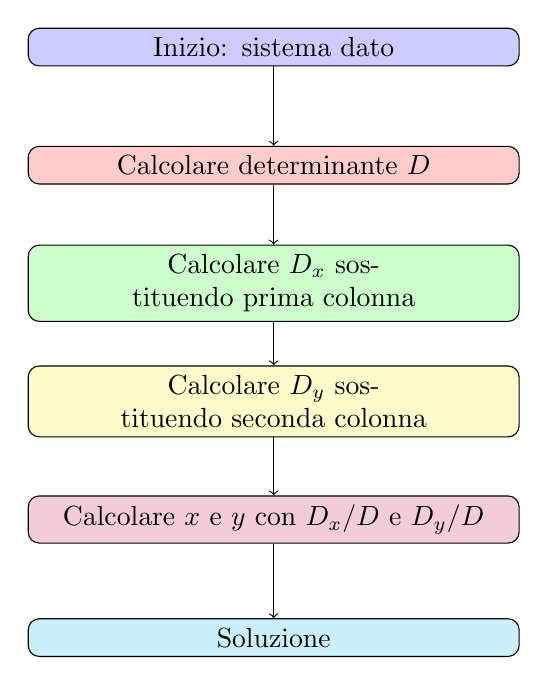
\begin{tikzpicture}[node distance=1.5cm, every node/.style={draw, rectangle, rounded corners, align=center, fill=blue!20, text width=6cm}]
        \node (start) {Inizio: sistema dato};
        \node (determinante) [below of=start, fill=red!20] {Calcolare determinante $D$};
        \node (det_x) [below of=determinante, fill=green!20] {Calcolare $D_x$ sostituendo prima colonna};
        \node (det_y) [below of=det_x, fill=yellow!20] {Calcolare $D_y$ sostituendo seconda colonna};
        \node (calcola) [below of=det_y, fill=purple!20] {Calcolare $x$ e $y$ con $D_x/D$ e $D_y/D$};
        \node (fine) [below of=calcola, fill=cyan!20] {Soluzione};
        
        \draw[->] (start) -- (determinante);
        \draw[->] (determinante) -- (det_x);
        \draw[->] (det_x) -- (det_y);
        \draw[->] (det_y) -- (calcola);
        \draw[->] (calcola) -- (fine);
    \end{tikzpicture}
\end{center}


\end{document}

